\documentclass[letterpaper,12pt]{texMemo}

\usepackage{graphicx}
\usepackage{setspace}
\usepackage{enumitem}
\usepackage{natbib}

\memoto{Future Students of ENGR-200W}
\memofrom{Partha Sarathi Ghosh}
\memosubject{My Thoughts on ENGR-200W}
\memodate{\today}
%\logo{\includegraphics[width=0.3\textwidth]{Microsoft-Logo.pdf}}

\begin{document}
\begin{singlespacing}
\setlist[enumerate]{itemsep=0mm}
\maketitle

% single or double spacing
%\doublespacing
% \begin{enumerate}
%     \item Identify all the physical and virtual assets in an organization.
%     \item Assign a risk profile to each asset.
%     \item Perform risk evaluation on each asset.
%     \item Perform risk mitigation on each asset.
% \end{enumerate}

% \begin{figure}[h!]
%     \centerline{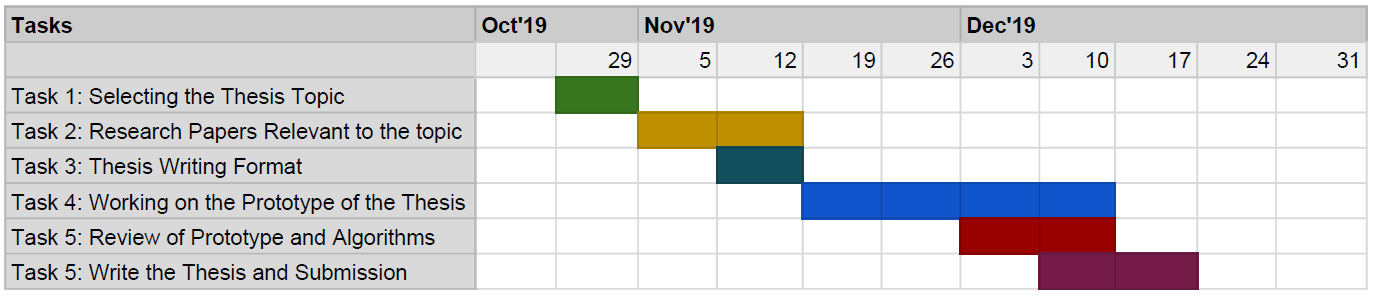
\includegraphics[scale=.45]{GaantChartThesis.PNG}}
%     \caption{Gantt Chart for Litearture Review}
%     %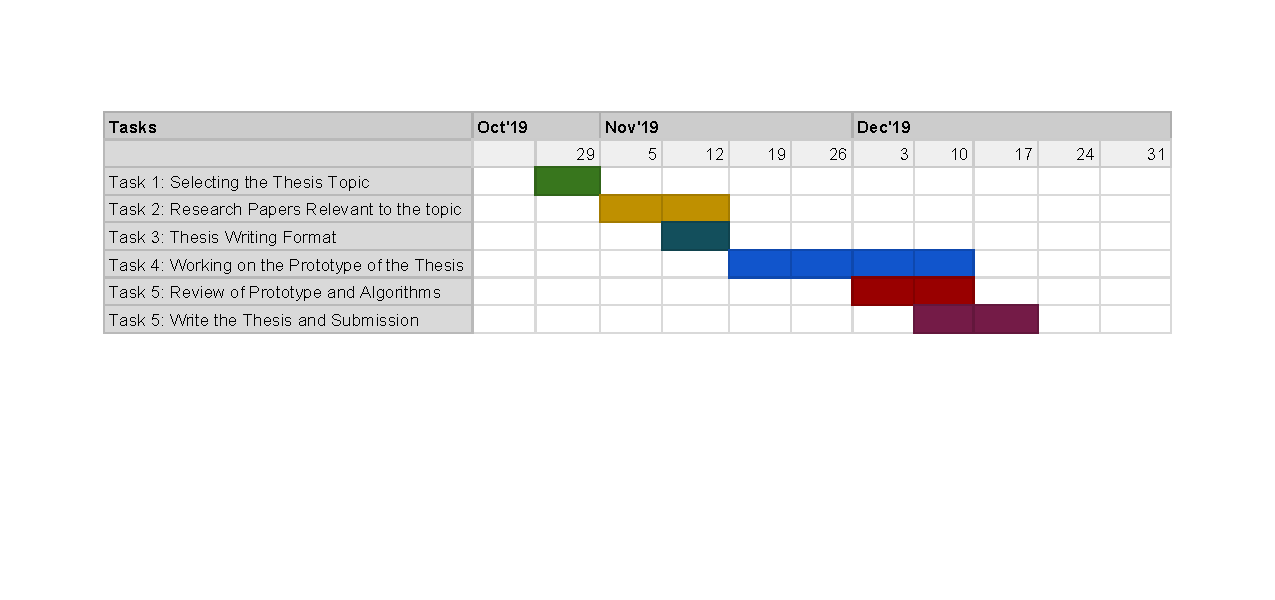
\includegraphics[scale=.8]{GaantChartThesis.pdf}
% \end{figure}

\section*{Purpose}
%This memo is for what ??
The purpose of this memo is to summarize my thoughts on the ENGR-200W course. The intended audience is my fellow students of San Jose State University (SJSU) who have signed up for the same course.


%%%%%%%%%%%%%%%%%%%%%%%%%%%%%%%
%PARTHA'S section starts here
%%%%%%%%%%%%%%%%%%%%%%%%%%%%%%%

\section*{Summary}
%%%%%%%%%%%%%%%%%%%%%%%%%%%%%%%
%PARTHA'S section starts here
%%%%%%%%%%%%%%%%%%%%%%%%%%%%%%%
In this memo I discuss my thoughts on the ENGR-200W course. I try to coalesce the Course Learning Objectives (CLOs), the assignments, and the methods of learning. I summarize the best practices learned from this course.

\section*{Discussion}

\subsubsection*{\textit{What is ENGR-200W Course?}}
ENGR-200W is a "Graduate level technical writing workshop designed to develop advanced communication skills that will readily transfer to the engineer's professional needs, along with research methodologies, copyright issues, and proper documentation for the master's thesis project" ~\citep{Infosjsu77:online}.
\subsubsection*{\textit{What are the CLOs of ENGR-200W?}}
The five CLOs of this course are:  
\begin{enumerate}
        \item Write using a variety of technical writing and professional formats. (CLO\#1)
        \item Compose with a clear focus on purpose, scope, and audience. (CLO\#2)
        \item Document properly and provide accurately formatted references. (CLO\#3)
        \item Locate and analyze information using a variety of research techniques (e.g., interviews, library, online searches). (CLO\#4)
        \item Demonstrate an understanding of the initial planning, brainstorming, and organizing a complex project. (CLO\#5)
\end{enumerate}
\subsubsection*{\textit{What are the methods of learning in ENGR-200W?}}
The text book for this course is "Technical Communication" ~\citep{markel_selber_2018}. This text book would be needed for reference during multiple assignments. There would be group assignments to complete various learning activities. These activities include "Common Errors" assignments, discussing social media policies of different companies and presenting them, etc. The "Common Errors" assignments would cover the common errors that we make while speaking and writing English. The course also focuses on presentation skills, both oral and using presentation materials. This course focuses on teaching students the art of creating effective presentations by using meaningful visuals along with public speaking skills.\\
There are plenty of writing assignments that need to be completed using different styles and formats, like, American Psychological Association (APA), Institute of Electrical and Electronics Engineers (IEEE), etc. These styles are commonly used to write technical documents. One of the SJSU library faculty members would also walk the students through the complex maze of technical articles.
\subsubsection*{\textit{Best Practices for ENGR-200W?}}
In this course, a student hones his/her writing skills. Writing includes creating your resume, a cover letter, reporting on a technical presentation, careful research on a trial thesis, analysis of a professional journal article, etc. Any written document needs to have clarity of its purpose, scope and the intended audience. Thus, planning is essential before you write anything. The articles need to cite the right sources for information accuracy and prevention of plagiarism. It is essential that the document is always proofread well to avoid grammar and spelling errors.\\ 
Do not procrastinate on the assignments; it is better if you start working on them early. Ask questions to the professor to clarify your doubts on the assignments. Be clear on the required document formats and styles. Being a good presenter is one of the key skills that one needs to develop to be successful in this course. So, practice public speaking. If you have stage fright, ask for advice from the professors.\\ 
Engage yourself in the class in all the "in class" activities. Whatever is your class size, you will end up with groups of people whom you have not worked with, and this will be a good time to develop the skills to work in a group. Be open to learning and have lots of fun. \\
Writing technical documents needs a lot of formatting styles and citations. Using a regular word processor can be cumbersome to cite and track references in the document. My advice would be to familiarize yourself with a \textit{simple, minimalistic, markup based type setting} tool like, \LaTeX{} ~\citep{LaTeXAdo7:online}. This type of tool will let you focus on the content and leave the formatting to templates. Use tools for grammar and spelling checks. This will make your proofreading faster. 

\section*{Conclusion}
This is the course which had the maximum number of assignments so far. I learned about writing purposeful, focussed, and targeted technical documents. I think I've been able to work on my presentation skills by receiving feedback and doing quite a few presentations in the class. 
%Before this class I read a T-shirt quote "English is important, but Engineering is importanter" and after ENGR-200W I would rewrite the quote to be "Engineering is important, but English is importanter".

%%%%%%%%%%%%%%%%%%%%%%%%%%%%%%%
%PARTHA'S section starts here
%%%%%%%%%%%%%%%%%%%%%%%%%%%%%%%
\bibliographystyle{apalike}
\bibliography{finalPreso}
\end{singlespacing}
\end{document}
